\documentclass[a4paper,12pt]{report}

\usepackage{alltt, fancyvrb, url,}
\usepackage{fancyhdr, graphicx}
\usepackage[utf8]{inputenc}
\usepackage{hyperref}

\usepackage[italian]{babel}

\usepackage[italian]{cleveref}
\renewcommand{\headrulewidth}{0pt}
\fancyhead[L]{}
\fancyhead[R]{
	
\includegraphics[width=4cm]{img/logocampus.jpg}
}
\pagestyle{plain}
\title{Relazione per \\``Programmazione di Reti'' \\ ChatGame}

\author{Carboni Leonardo - Ongaro Andrea}
\date{\today}


\begin{document}

\maketitle

\tableofcontents
\thispagestyle{fancy}

\chapter{Traccia Scelta}
Sfruttando il principio della CHAT vista a lezione implementate un’architettura client-server per il supporto di un Multiplayer Playing Game testuale. \\
I giocatori che accedono alla stanza sono accolti dal Master (server) che assegna loro un ruolo e propone loro un menu con tre opzioni, due delle quali celano una domanda mentre la terza è l’opzione trabocchetto. Se sceglie l’opzione trabocchetto viene eliminato dal gioco e quindi esce dalla chat.
Se seleziona invece una delle domande e risponde correttamente al quesito acquisisce un punto, in caso contrario perde un punto.\\
Il gioco ha una durata temporale finita; il giocatore che al termine del tempo ha acquisito più punti è il vincitore

\chapter{Descrizione Generale}
In questo capitolo esponiamo la nostra interpretazione della traccia scelta tra le tre proposte soffermandoci anche sulle scelte di progettazione più rilevanti.

\subsection{Preparativi}
Dopo aver aperto le connessioni ai client, essi saranno liberi di accedere al server il quale accetterà tutte le connessioni in entrata. Quando la connessione è stata accettata il client aprirà una finestra nella quale bisognerà inserire il nome del giocatore e cliccare il tasto invio. Alla pressione di quest'ultimo l'istanza del client invierà un messaggio al server contenente il nome specificato. \\
Nel caso in cui fosse specificato un nome già presente nella lista dei giocatori, a quest'ultimo verrà aggiunto un \_ finale mentre se il gioco fosse già iniziato verrà segnalato all'utente e verrà messo in una lista d'attesa dove non dovrà compiere nessuna azione.\\
All'apertura della seconda schermata (il gioco vero e proprio), verranno mostrati i nomi dei giocatori presenti seguiti dai corrispettivi ruoli, le istruzioni del gioco e il ruolo del giocatore appena entrato.\\
Per ogni giocatore già presente nel server verrà mostrato un messaggio che specifica l'aggiunta nuovo giocatore, anch'esso a sua volta seguito dal ruolo corrispondente. \\
Quando tutti i giocatori presenti nella lobby esprimeranno la loro intenzione di giocare tramite il tasto "Pronto" o il comando "\{start\}"
il server manderà un messaggio broadcast specificando il turno e la domanda di scelta della porta.\clearpage

Il gioco non può partire solamente in tre casi:
\begin{itemize}
	\item la presenza di un solo giocatore all'interno del gioco, anche se si è dichiarato pronto
	\item non tutti i giocatori si sono dichiarati pronti
	\item il gioco è già partito
\end{itemize}
Una volta che la partita è iniziata nessun giocatore potrà entrare e solamente il giocatore corrente potrà inviare messaggi - se un altro utente scriverà un messaggio verrà avvertito che non è il suo turno ma il messaggio appena scritto verrà comunque inoltrato agli altri giocatori.\\
Verrà tenuta traccia anche dei turni giocati dove un turno corrisponde alla completa iterazione dei giocatori ancora in gioco.\clearpage

\subsection{Il Gioco}
Il gioco ha una durata complessiva massima di 180 secondi (3 minuti), al termine dei quali verrà stampata la classifica.\\
Vengono poi mostrate tre possibili porte tra le quali il giocatore corrente potrà scegliere. Due di queste saranno giuste e mostreranno una domanda presa casualmente tra quelle inserite nel file "domande.json" mentre una terza porta ha al suo interno una bomba.\\
Se il giocatore sceglierà la porta con al suo interno la bomba, questo verrà espulso dalla partita e segnalato come morto, rimanendo comunque all'interno della chat per osservare il proseguimento del gioco e eventualmente iniziare un'altra partita.\\
Se il giocatore sceglierà una delle due porte non contenenti la bomba gli verrà posta una domanda e verrà attivato un timer secondario di 5 secondi. In caso il giocatore scegliesse la risposta errata o il countdown terminasse, gli verranno sottratti 100 punti.\\
Nel caso di risposta corretta verranno aggiunti al punteggio attuale del giocatore 100 punti moltiplicati per il turno corrente così da ricevere più punti in funzione della durata della partita.\\

\subsection{Fine Gioco}
Il gioco terminerà in tre casi:
\begin{itemize}
	\item un giocatore rimarrà da solo 
	\item al termine del countdown impostato all'inizio del gioco.\\ In questo caso verranno analizzati tutti i giocatori ancora all'interno del gioco e verrà mostrato il giocatore che ha realizzato più punti
	\item all'uscita di uno dei giocatori
\end{itemize}
Dopo aver mostrato la classifica verranno impostati tutti i giocatori come non pronti e verrà chiesto di giocare un'altra partita. In questa fase potranno entrare anche altri giocatori e verranno spostati i giocatori dalla sala d'attesa alla lista dei giocatori partecipanti.\clearpage

\begin{figure}[h]
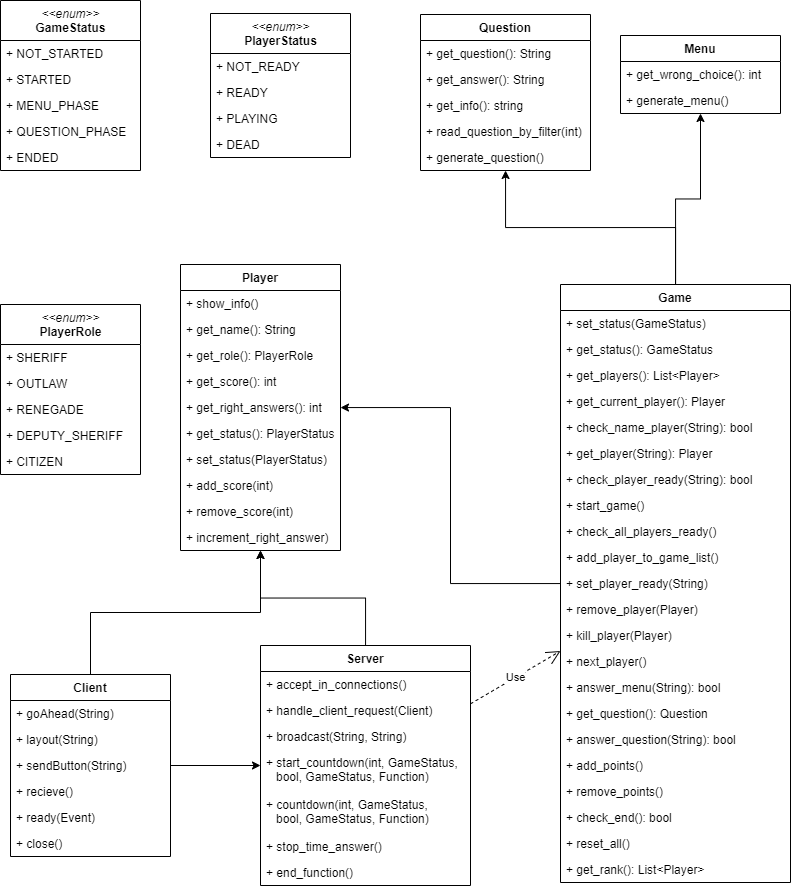
\includegraphics[width=\textwidth,height=\textheight,keepaspectratio]{img/uml.jpg}
\caption{Schema UML dell'analisi del problema, con rappresentate le entità principali ed i rapporti fra loro}
\end{figure}

\chapter{Strutture dati}
Abbiamo utilizzato alcune delle strutture dati offerte da python preferendole rispetto ad altre.
\subsection{Dizionari}
Innanzitutto sono stati utilizzati i dizionari, un tipo built-in, mutabile e non ordinato che contiene elementi formati da una chiave (key) e un valore (value). Una volta che il dizionario è creato viene popolato con un insieme di coppie <chiave, valore>, si può usare la chiave (che deve essere univoca) per ottenere il valore corrispondente.\\
É proprio per queste caratteristiche che sono stati utilizzati per implementare la memorizzazione degli utenti che accedono al server e per la lettura da file. Un dizionario viene utilizzato per la registrazione dei client in ingresso mentre il secondo per i nomi associati agli indirizzi. Ogni elemento corrisponderà al nome dell'utente che viene identificato da un indirizzo ip.\\
Il terzo e ultimo dizionario verrà creato dal metodo json.load, utilizzato dopo aver importato la libreria interna di python "json".
Questo metodo ha il compito di leggere il file passato in input, analizzare il contenuto JSON e creare un dizionario con i dati.\clearpage
 
\subsection{Liste} 
Una lista è una serie ordinata di valori, ognuno identificato da un indice. I valori che fanno parte della lista sono chiamati elementi.\\
Sono state utilizzate le liste perché al contrario delle tuple presenti nei dizionari, che contengono oggetti eterogenei tra loro, riescono a contenere istanze di oggetti omogenei tra loro. Per quanto riguarda i set sono stati scartati per l'impossibilità di garantire un ordine al loro interno, cosa molto importante per la realizzazione della logica di gioco.\\
Le liste vengono usate per immagazzinare
\begin{itemize}
	\item i dizionari con le informazioni delle domande ottenute dal corrispettivo file.
	\item i giocatori che stanno giocando 
	\item i giocatori che sono entrati dopo che il gioco era iniziato
\end{itemize}

\subsection{Enums}
Sono stati usati multipli enum per definire i vari stati del gioco e del giocatore e i suoi ruoli.

\chapter{Threads attivati}
\subsection{Gioco principale}
All'interno del gioco principale vengono creati dei thread per la gestione del tempo totale di gioco, ovvero 3 minuti e per il tempo di risposta del giocatore (5 secondi). Quest'ultimo thread viene attivato ogni volta che un giocatore deve rispondere ad una domanda e viene fatto per evitare che perda troppo tempo nel rispondere così da togliere l'opportunità di giocare agli altri utenti.

\subsection{Server}
Nel server vengono gestiti due thread. Il primo si occupa di accettare le connessioni in entrata che grazie al ciclo while rimangono in attesa occupandosi di immagazzinare tutti i client arrivati. Il secondo, invece, ha il compito di gestire i client e tutta la logica di gioco. Il suo unico parametro è il client che deve gestire in modo tale da poter ottenere i messaggi che invia. A seconda del messaggio che invierà l'utente verrà eseguita una diversa azione.
Per far sì che il server non si chiuda subito dopo essere partito, ovvero dopo l'accettazione delle connessioni, utilizziamo il metodo join che aspetta per il completamento della funzione senza passare alla riga successiva. Facendo diversamente causeremmo la chiusura del server.

\subsection{Client}
Per quanto riguarda il client viene utilizzato un unico thread che si occupa di gestire la ricezione dei messaggi andando poi ad aggiungerli alla vista che si occupa di mostrarli, realizzata tramite la libreria tkinter.

\chapter{Struttura del progetto}
É stato scelto di strutturare il progetto "a oggetti" per integrare le conoscenze acquisite nel corso "Programmazione ad Oggetti" e sfruttare al massimo le potenzialità del linguaggio.

\subsection{Roadmap}
\begin{itemize}
	\item \textbf{Root folder/src}: contiene la classe Server e tutte le sottocartelle,
	\item \textbf{Client}: contiene la classe Client,
	\item \textbf{Game}: contiene la classe Game e l'enum GameStatus,
	\item \textbf{Player}: contiene la classe Player e gli enum PlayerRole e PlayerStatus,
	\item \textbf{Menu}: contiene la classe Menu.
\end{itemize}
All'interno dei vari file è presente una ampia documentazione sul loro funzionamento.
\chapter{Indicazioni per la loro esecuzione}
\subsection{Eseguire il Server}
\begin{verbatim}
	python3 server.py
\end{verbatim}
Il server inizierà ad ascoltare sul'IP "\textbf{127.0.0.1}" e la porta "\textbf{53000}". Per modificare questi valori occorre modificare direttamente il file.
\subsection{Eseguire un Client}
Spostarsi all'interno del client utilizzando le apposite istruzioni del sistema utilizzato per far partire il gioco.
\begin{verbatim}
	python3 client.py
\end{verbatim}
Il client proverà automaticamente a connettersi all'IP "\textbf{127.0.0.1}" e alla porta "\textbf{53000}". Per modificare questi valori occorre modificare direttamente il file.
\subsection{Istruzioni di gioco}
Le istruzioni di gioco sono ampiamente specificate all'interno dei precedenti capitoli.
\end{document}
